\section{Methodology}
\begin{figure*}[h!/0]
    \centering
    \includegraphics[scale=0.3]{images/Screenshot from 2023-11-08 15-32-25.png}
    \caption{Analysis Process Flowchart}
    \label{fig:Analysis Process Flowchart}
\end{figure*}
\subsection{Data}
Our Segformer model underwent training utilizing the dataset provided by Mindboggle-101 via their open science framework \cite{10.3389/fnins.2012.00171}. This dataset comprises T1-weighted MRI images, along with man-made volumetric labels that correspond to distinct cerebral regions. Subsequently, the Segformer model was subjected to testing using patient data sourced from the Parkinson's Progression Markers Initiative (PPMI) database \cite{PPMI}. This patient dataset includes T1-weighted MRI images, DaTSCAN SPECT images, and comprehensive baseline cohort information for each patient. The image pre-processing workflow for both training and testing phases of our model is elucidated in Figure 2. Regarding the Mindboggle MRI data, these images were already skull stripped and conformed to the Montreal Neurological Institute (MNI) coordinate system. Subsequently, a Z-score normalization technique was applied to standardize pixel value distributions. \\
\textbf{Z-score Normalization} is a technique that scales the values of a feature to have a mean of 0 and a standard deviation of 1. This initial step is crucial to standardize all MRI images which were taken across various systems. The formula for Z-score normalization of a pixel, $x$, is:
\begin{equation}
 x_{new} = \frac{x-\mu}{\sigma}
\end{equation}
where $x_{new}$ is the new value for the pixel, $\mu$ is the average value of the MRI, and $\sigma$ is the standard deviation of the MRI.\\
\textbf{Absolute discretization} is a preprocessing technique that takes in an MRI with a continuous range of values and assigns each pixel to a discrete bin, where the number of bins is predefined. Literature has shown that absolute discretization boosts radiomic feature extraction for MRI images \cite{10.1371/journal.pone.0213459}. For the Segformer preprocessing, a bin size of 256 was used to cover the range of grayscale. The formula for absolute discretization is below:
\begin{equation}
 x_{new} = 256 * \frac{x-x_{min}}{x_{max}-x_{min}}
\end{equation}
then $x_{new}$ is converted into an integer, assigning it to a bin.\\
\textbf{Gaussian noise} was introduced to the MRI images to add a controlled level of real-world noise. Upon observation, the Mindboggle dataset was cleaner than its PPMI counterpart. Since the weights trained off of Mindboggle are applied to PPMI for segmentation, the noise was added to bring the two datasets more in line and allow the Segformer model to account for noisy inputs. The formula for adding Gaussian noise is below:
\begin{equation}
 x_{new} = x + \mathcal{N}(0,3)
\end{equation}
These 3D volumetric images were then converted into 2D slices in the axial, sagittal, and coronal planes, facilitating their input into the Segformer model for training.\\
\textbf{Skull-stripping} of the PPMI MRI images were done using the Robex package \cite{iglesias2011robust}. The Robex method combines a Random Forest classifier to detect the brain-skull boundary and a point distribution model to guarantee the result is possible.\\
\textbf{The MNI Coordinate System} is a commonly used coordinate system for brain MRI analysis and the one used by PPMI for their DaTSCAN images. Each coordinate in the MNI system aligns to a specific location in the brain. The coordinate (0,0,0) lies center in the brain with the right hemisphere, front of brain, and top of brain being the positive direction for the x,y, and z axis respectively. 


MRI template using an affine transformation. Following alignment, the MRI images were subjected to Z-score normalization and absolute discretization to ensure alignment with the training data. They were then segmented into 2D slices within the axial, sagittal, and coronal planes before being incorporated into the model.

For DaTSCAN images, they were matched with MRI images taken at the closest time point within a year. These DaTSCAN images were already aligned with the MNI coordinate system but were upscaled to match the dimensions of the MRI images, resulting in a uniform size of (182, 218, 182). Each image pair was subsequently assigned a patient state label using information from PPMI's CONCOHORT section.
\subsection{Segformer}
\begin{figure*}[h!]
    \centering
    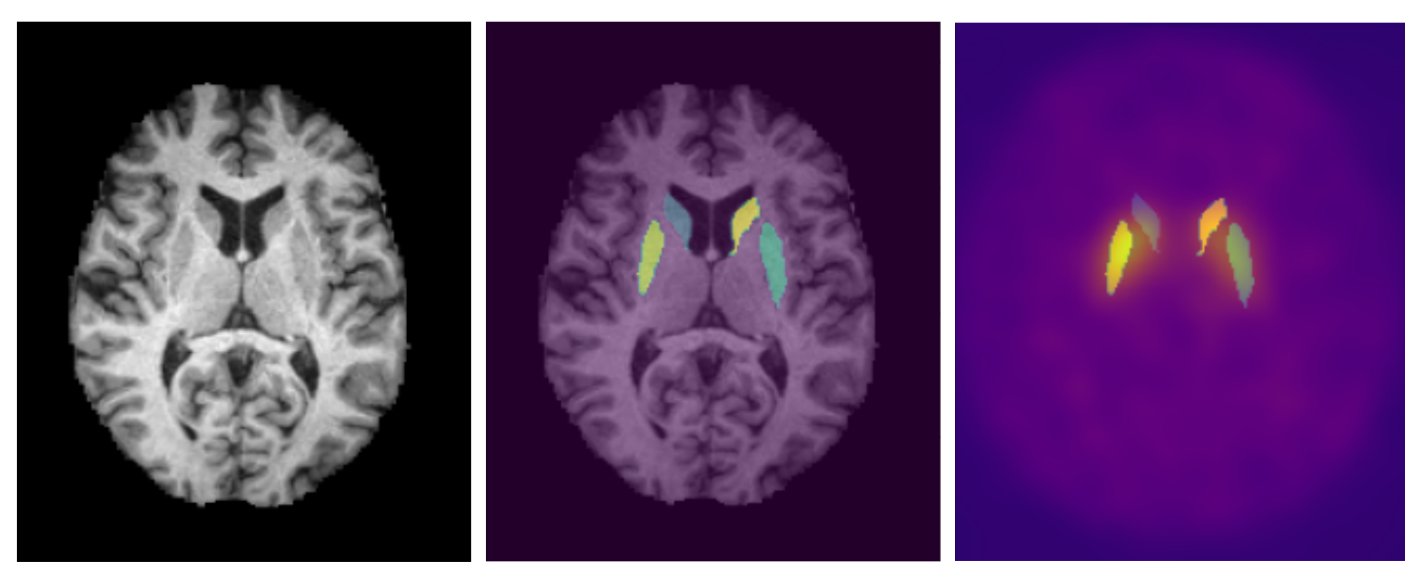
\includegraphics[scale=0.3]{images/3Images.png}
    \caption{Overview of Segformer Process. a) T1-Weighted MRI b) Mask generated from Segformer overlaid on MRI c) Mask generated from Segformer overlaid on DaTSCAN}
    \label{fig:Analysis Process Flowchart}
\end{figure*}